%//==============================--@--==============================//%
\clearpage
\section{Reflexão e Refração}

%//==============================--@--==============================//%
\subsection{Condições de Fronteira}
\label{sec:boundary-conditions-waves}

As condições de fronteira para os campos eletromagnéticos na interação entre dois meios materiais são dadas abaixo:

\begin{figure}[H]
    \centering
    \begin{minipage}[c]{0.25\linewidth}
        $$
            \boxed{%
                \begin{aligned}
                    \mathbf{E}_{1t} - \mathbf{E}_{2t} &= 0 \\
                    \mathbf{H}_{1t} - \mathbf{H}_{2t} &= \mathbf{J}_{s} \times \mathbf{\hat{n}} \\
                    \mathbf{D}_{1n} - \mathbf{D}_{2n} &= \rho_{s} \\
                    \mathbf{B}_{1n} - \mathbf{B}_{2n} &= 0
                \end{aligned}
            }
        $$
    \end{minipage}\hspace{1em}
    \begin{minipage}[c]{0.55\linewidth}
        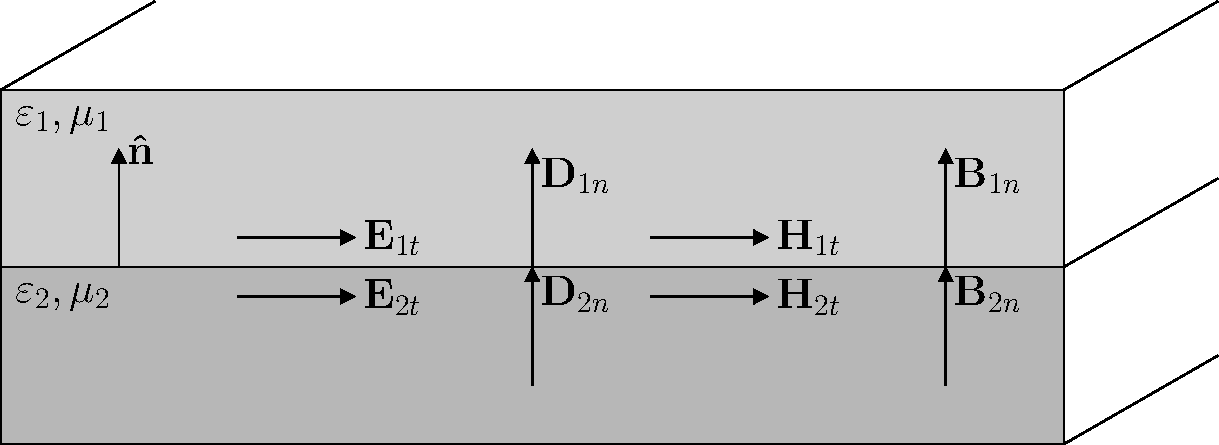
\includegraphics[width=0.925\linewidth]{img/1/Material-interface.pdf}
    \end{minipage}
    \caption{Condições de fronteira entre dois meios materiais}
    \label{fig:Material-interface}
\end{figure}

\vspace{-1em}
onde $\mathbf{\hat{n}}$ é um vetor unitário normal à fronteira (ou interface), que aponta do meio-2 para o meio-1.

As quantidades $\rho_s, \mathbf{J}_s$ são quaisquer \textit{cargas de superfície externas} e \textit{densidades de corrente de superfície} na superfície de fronteira e são medidas em unidades de $[\text{C/m}^2]$ e $[\text{A/m}]$.

Cada vetor pode ser decomposto como a soma de uma parte tangencial à superfície e uma parte perpendicular a ela, isto é, $\mathbf{E} = \mathbf{E}_t + \mathbf{E}_n$. Utilizando a identidade vetorial,
$$
    \mathbf{E} = \mathbf{\hat{n}} \times (\mathbf{E} \times \mathbf{\hat{n}}) + \mathbf{\hat{n}}(\mathbf{\hat{n}} \cdot \mathbf{E}) = \mathbf{E}_t + \mathbf{E}_n
$$
identificamos estas duas partes como:
$$
    \mathbf{E}_t = \mathbf{\hat{n}} \times (\mathbf{E} \times \mathbf{\hat{n}}), \quad \mathbf{E}_n = \mathbf{\hat{n}} (\mathbf{\hat{n}} \cdot \mathbf{E})
$$
Por outras palavras, as componentes \textit{tangenciais} do campo $\mathbf{E}$ são contínuas através da interface; a diferença das componentes \textit{tangenciais} do campo $\mathbf{H}$ são iguais às densidades de corrente da superfície; a diferença das componentes \textit{normais} da densidade de fluxo $\mathbf{D}$ são iguais à densidade de carga da superfície; e as componentes \textit{normais} da densidade de fluxo magnético $\mathbf{B}$ são contínuas.

\begin{warning}
    É relevante salientar que a continuidade dos campos tangenciais numa interface garante a continuidade da componente normal do vetor de Poynting na interface, se considerarmos $\mathbf{J}_{s} = 0$ temos:
    $$
        \mathbf{S}_1 \cdot \mathbf{\hat{n}} = (\mathbf{E}_1 \times \mathbf{H}_1) \cdot \mathbf{\hat{n}} = (\mathbf{E}_{1t} \times \mathbf{H}_{1t}) \cdot \mathbf{\hat{n}} = (\mathbf{E}_{2t} \times \mathbf{H}_{2t}) \cdot \mathbf{\hat{n}} = \mathbf{S}_2 \cdot \mathbf{\hat{n}}.
    $$
    Isto é, a interface não pode absorver a energia da onda.
\end{warning}

\begin{warning}
    É relevante analisar as condições de fronteira numa interface com um condutor elétrico perfeito (PEC)~\cite{silveirinha2023}. Um condutor elétrico perfeito é um material idealizado com condutividade elétrica $\sigma \to +\infty$. Como a corrente de condução é $\mathbf{J}_{\text{cond}} = \sigma \mathbf{E}$, o campo elétrico dentro de um condutor perfeito deve anular-se. Assim, um material PEC ideal comporta-se como um espelho perfeito e é impenetrável pela luz. Consequentemente, o campo elétrico na interface com um material PEC deve desaparecer:
    $$
        \mathbf{E}_{1t} = \mathbf{E}_{2t} = 0
        \quad \text{(interface PEC)}
    $$
    Note-se que o campo magnético tangencial $\mathbf{H}_{1t}$ (avaliado fora do material) não desaparece. Determina uma densidade de corrente de superfície na fronteira do PEC.
\end{warning}

%//==============================--@--==============================//%
\subsection{Incidência em Interfaces Planas}

Nesta secção focamos a nossa atenção na incidência de ondas planas em interfaces que separam dois meios materiais.

\subsubsection{Incidência Normal}

A direção de propagação da onda incidente, $\mathbf{\hat{d}}^i$, é perpendicular à superfície da interface. Nestes moldes, os campos da onda incidente são:
\begin{equation}
    \mathbf{\underline{E}}^{\text{inc}} = \mathbf{\underline{E}}^{\text{inc}}_{0}\, e^{-\gamma_1 \mathbf{\hat{d}}^i \cdot \mathbf{r}},
    \qquad
    \mathbf{\underline{H}}^{\text{inc}} = \frac{1}{\eta_1} \mathbf{\hat{d}}^i \times \mathbf{\underline{E}}^{\text{inc}}_{0}\, e^{-\gamma_1 \mathbf{\hat{d}}^i \cdot \mathbf{r}}
\end{equation}
através das relações apresentadas \ref{sec:ondas-com-perdas}.

\begin{figure}[H]
    \centering
    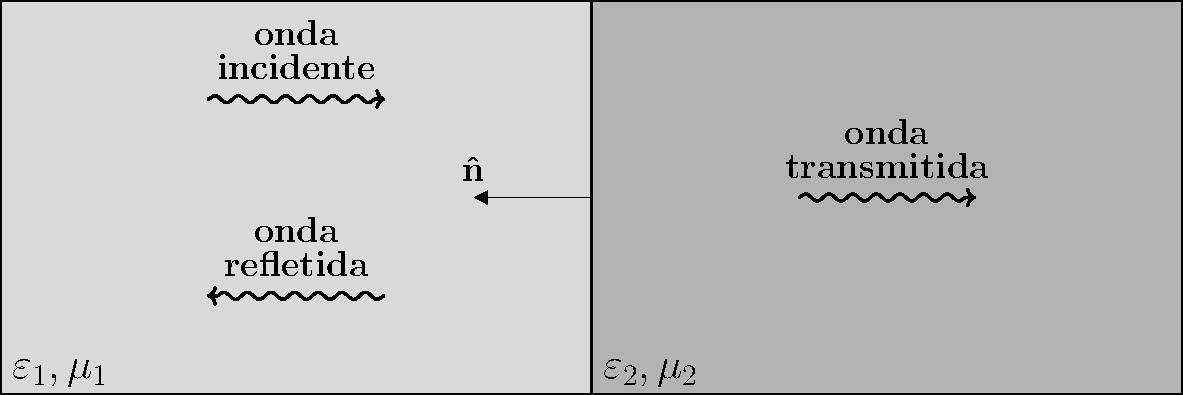
\includegraphics[width=0.5\linewidth]{img/1/Incidencia-normal.pdf}
    \caption{Incidência normal numa interface plana}
    \label{fig:Incidencia-normal}
\end{figure}

\vspace{-1em}
Como seria de esperar intuitivamente, a onda incidente irá gerar uma onda transmitida no meio 2 e uma onda refletida no meio 1, com direções de propagação $\mathbf{\hat{d}}^t = \mathbf{\hat{d}}^i$ e $\mathbf{\hat{d}}^r = -\mathbf{\hat{d}}^i$. Podemos escrever os campos respetivos:
\begin{equation}
    \mathbf{\underline{E}}^{\text{ref}} = \mathbf{\underline{E}}^{\text{ref}}_{0}\, e^{-\gamma_1 \mathbf{\hat{d}}^r \cdot \mathbf{r}},
    \qquad
    \mathbf{\underline{H}}^{\text{ref}} = \frac{1}{\eta_1} \mathbf{\hat{d}}^r \times \mathbf{\underline{E}}^{\text{ref}}_{0}\, e^{-\gamma_1 \mathbf{\hat{d}}^r \cdot \mathbf{r}}
\end{equation}
\begin{equation}
    \mathbf{\underline{E}}^{\text{tx}} = \mathbf{\underline{E}}^{\text{tx}}_{0}\, e^{-\gamma_2 \mathbf{\hat{d}}^t \cdot \mathbf{r}},
    \qquad
    \mathbf{\underline{H}}^{\text{tx}} = \frac{1}{\eta_1} \mathbf{\hat{d}}^t \times \mathbf{\underline{E}}^{\text{tx}}_{0}\, e^{-\gamma_2 \mathbf{\hat{d}}^t \cdot \mathbf{r}}
\end{equation}

Estes campos obdecem às condições de fronteira anunciadas \hyperref[sec:boundary-conditions-waves]{anteriormente}, uma vez que as ondas planas são transversais\footnote{Nesta situação, $\mathbf{\underline{E}}$ e $\mathbf{\underline{H}}$ são paralelos (tangenciais) à interface.}, i.e.,
\begin{equation}
    \begin{aligned}
        \mathbf{\underline{E}} =
        \begin{cases}
            \mathbf{\underline{E}}^{\text{inc}} + \mathbf{\underline{E}}^{\text{ref}} & \text{antes da interface} \\
            \mathbf{\underline{E}}^{\text{tx}} & \text{depois da interface}
        \end{cases}
        \qquad\quad
        \mathbf{\underline{H}} = 
        \begin{cases}
            \mathbf{\underline{H}}^{\text{inc}} + \mathbf{\underline{H}}^{\text{ref}} & \text{antes da interface} \\
            \mathbf{\underline{H}}^{\text{tx}} & \text{depois da interface}
        \end{cases}
    \end{aligned}
\end{equation}
que se reduz às relações:
\begin{equation} \label{eq:1.72}
    \mathbf{\underline{E}}^{\text{inc}} + \mathbf{\underline{E}}^{\text{ref}} = \mathbf{\underline{E}}^{\text{tx}},
    \qquad
    \frac{1}{\eta_1}\mathbf{\hat{d}}^i \times (\mathbf{\underline{E}}^{\text{inc}} - \mathbf{\underline{E}}^{\text{ref}}) = \frac{1}{\eta_2}\mathbf{\hat{d}}^i \times \mathbf{\underline{E}}^{\text{tx}}
\end{equation}
Removendo o produto externo da segunda relação, vem que
\begin{equation}
    \mathbf{\underline{E}}^{\text{inc}} + \mathbf{\underline{E}}^{\text{ref}} = \mathbf{\underline{E}}^{\text{tx}},
    \qquad
    \frac{1}{\eta_1} (\mathbf{\underline{E}}^{\text{inc}} - \mathbf{\underline{E}}^{\text{ref}}) = \frac{1}{\eta_2} \mathbf{\underline{E}}^{\text{tx}}.
\end{equation}
É conveniente definir a componente refletida e transmitida em função da componente incidente:
\begin{equation}
    \mathbf{\underline{E}}^{\text{ref}} = \rho \mathbf{\underline{E}}^{\text{inc}}
    \qquad
    \mathbf{\underline{E}}^{\text{tx}} = \tau \mathbf{\underline{E}}^{\text{inc}}
\end{equation}
onde $\rho$ é definido como coeficiente de reflexão e $\tau$ como coeficiente de transmissão. Da equação \ref{eq:1.72}, vem que
\begin{equation}
    \boxed{%
        \rho = \frac{\eta_2 - \eta_1}{\eta_1 + \eta_2}
    }
    \qquad\quad
    \boxed{%
        \tau = 1 + \rho = \frac{2\eta_2}{\eta_1 + \eta_2}
    }
\end{equation}
\textbf{Nota}: As componentes do campo são avaliadas na interface!

\begin{warning}
    \begin{itemize}
        \item  Quando as impedâncias dos dois materiais são idênticas ($\eta_2 = \eta_1$), não há onda refletida e a onda incidente é totalmente transmitida para o segundo meio. Neste caso, diz-se que os materiais estão ``adaptados''.
        
        \item A situação oposta ocorre quando o meio 2 é um condutor elétrico perfeito (PEC). Como a impedância intrínseca de um condutor perfeito desaparece ($\eta_{PEC} = \eta_2 = 0$), o coeficiente de reflexão nesse caso torna-se $\rho_{\text{PEC}} = -1$. Isso confirma que um condutor perfeito comporta-se como um espelho perfeito.    
    \end{itemize}
\end{warning}

%//==============================--@--==============================//%
\subsubsection{Incidência Oblíqua}

Numa situação mais geral, a onda incidente poderá atingir a interface numa direção oblíqua. Neste caso, é necessário ter em consideração o ângulo de incidência $\theta_i$, de reflexão $\theta_r$ e de transmissão $\theta_t$. Isto pode ser feito à custa do vetor unitário normal à interface, $\mathbf{\hat{n}}$.
\begin{equation}
    -\mathbf{\hat{d}}^i \cdot \mathbf{\hat{n}} = \cos \theta_i
    \qquad
    \mathbf{\hat{d}}^r \cdot \mathbf{\hat{n}} = \cos \theta_r
    \qquad
    \mathbf{\hat{d}}^t \cdot \mathbf{\hat{n}} = \cos \theta_t
\end{equation}
Definimos também o \emph{plano de incidência}, gerado pelos vetores $\mathbf{\hat{d}}^i$ e $\mathbf{\hat{n}}$.

\begin{figure}[H]
    \centering
    \begin{subfigure}[c]{0.55\linewidth}
        \centering
        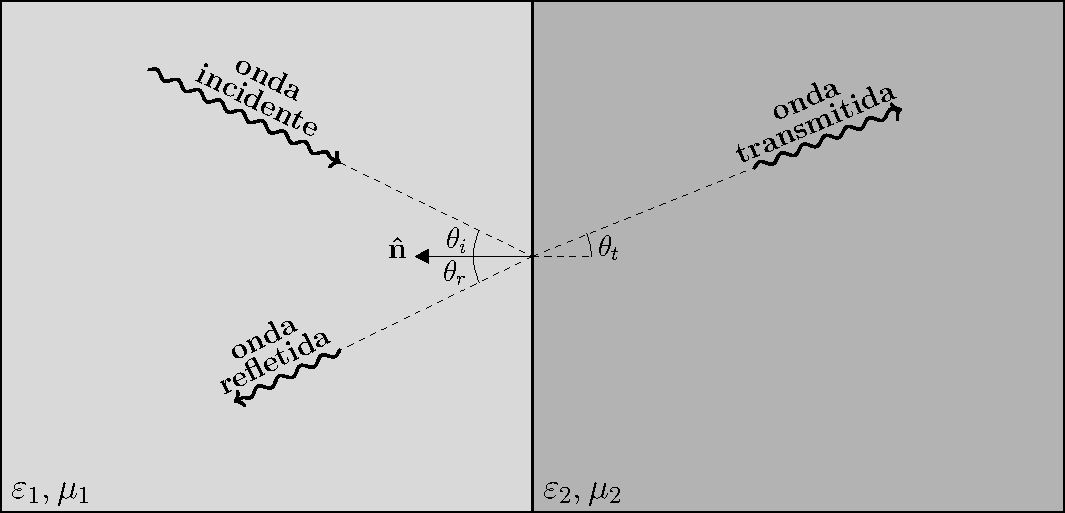
\includegraphics[width=\linewidth]{img/1/Incidencia-obliqua.pdf}
        \caption{Interação entre dois meios}
    \end{subfigure}\hfil
    \begin{subfigure}[c]{0.2\linewidth}
        \centering
        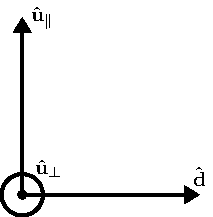
\includegraphics[width=\linewidth]{img/1/Vetores-unitarios.pdf}
        \caption{Relação entre os vetores unitários, $\mathbf{\hat{u}}_{\parallel} \times \mathbf{\hat{u}}_{\perp} = \mathbf{\hat{d}}$.}
    \end{subfigure}
    \caption{Incidência oblíqua numa interface plana}
    \label{fig:Incidencia-obliqua}
\end{figure}

\vspace{-1em}
Uma vez que os campos da onda incidente oscilam num plano transversal a $\mathbf{\hat{d}}^i$ ($\mathbf{E}^{\text{inc}} \cdot \mathbf{\hat{d}}^i = 0$), é conveniente introduzir dois vetores unitários, $\mathbf{\hat{u}}_{\parallel}$ e $\mathbf{\hat{u}}_{\perp}$, que geram este plano. Por construção, os vetores unitários cumprem a seguinte condição:
\begin{equation}
    \mathbf{\hat{u}}^{i}_{\parallel} \times \mathbf{\hat{u}}_{\perp} = \mathbf{\hat{d}}^i
\end{equation}
Note-se que o vetor $\mathbf{\hat{u}}_{\perp}$ é perpendicular ao plano de incidência, enquanto o vetor $\mathbf{\hat{u}}^{i}_{\parallel}$ é paralelo ao plano de incidência, de acordo com as notações. 

O campo incidente pode ser escrito em termos de $\mathbf{\hat{u}}_{\parallel}$ e $\mathbf{\hat{u}}_{\perp}$ da seguinte forma:
\begin{equation}
    \mathbf{\underline{E}}^{\text{inc}} = \underline{\mathrm{E}}^{i}_{\parallel} \mathbf{\hat{u}}^{i}_{\parallel} + \underline{\mathrm{E}}^{i}_{\perp} \mathbf{\hat{u}}_{\perp}
\end{equation}
onde as componentes $\underline{\mathrm{E}}^{i}_{\parallel}$ e $\underline{\mathrm{E}}^{i}_{\perp}$ são as componentes paralela e perpendicular do campo, respetivamente.

Uma construção similar pode ser feita para os campos $\mathbf{\underline{E}}^{\text{ref}}$ e $\mathbf{\underline{E}}^{\text{tx}}$,
\begin{equation}
    \mathbf{\hat{u}}^{r}_{\parallel} \times \mathbf{\hat{u}}_{\perp} = \mathbf{\hat{d}}^r
    \qquad\qquad
    \mathbf{\hat{u}}^{t}_{\parallel} \times \mathbf{\hat{u}}_{\perp} = \mathbf{\hat{d}}^t
\end{equation}
que leva às decomposições seguintes:
\begin{equation}
    \mathbf{\underline{E}}^{\text{ref}} = \underline{\mathrm{E}}^{r}_{\parallel} \mathbf{\hat{u}}^{r}_{\parallel} + \underline{\mathrm{E}}^{r}_{\perp} \mathbf{\hat{u}}_{\perp}
    \qquad\qquad
    \mathbf{\underline{E}}^{\text{tx}} = \underline{\mathrm{E}}^{t}_{\parallel} \mathbf{\hat{u}}^{t}_{\parallel} + \underline{\mathrm{E}}^{t}_{\perp} \mathbf{\hat{u}}_{\perp}
\end{equation}

%//==============================--@--==============================//%
\subsubsection{Lei de Snell}
\label{subsubsec:lei-de-snell}

Nesta secção viramos a nossa atenção para o ângulo de incidência $\theta_i$ e o ângulo de transmissão $\theta_t$. Podemos relacionar estes ângulos através das \hyperref[sec:boundary-conditions-waves]{condições de fronteira} já enunciadas.

Os campos associados às ondas planas incidentes, refletidas e transmitidas são:
\begin{equation}
    \mathbf{\underline{E}}^{\text{inc}} = \mathbf{\underline{E}}^{\text{inc}}_{0}\, e^{-\gamma_1 \mathbf{\hat{d}}^i \cdot \mathbf{r}}
    \qquad
    \mathbf{\underline{E}}^{\text{ref}} = \mathbf{\underline{E}}^{\text{ref}}_{0}\, e^{-\gamma_1 \mathbf{\hat{d}}^r \cdot \mathbf{r}}
    \qquad
    \mathbf{\underline{E}}^{\text{tx}} = \mathbf{\underline{E}}^{\text{tx}}_{0}\, e^{-\gamma_2 \mathbf{\hat{d}}^t \cdot \mathbf{r}}
\end{equation}
Impõe-se a continuidade das componentes do campo tangentes à interface e verifica-se que:
\begin{equation}
    \left[ \mathbf{\underline{E}}^{\text{inc}} + \mathbf{\underline{E}}^{\text{ref}} \right] \cdot \mathbf{\hat{t}} = \mathbf{\underline{E}}^{\text{tx}} \cdot \mathbf{\hat{t}}
    \quad\iff\quad
    \left[ \mathbf{\underline{E}}_{0}^{\text{inc}} e^{-\gamma_1 \mathbf{\hat{d}}^i \cdot \mathbf{r}} + \mathbf{\underline{E}}_{0}^{\text{ref}} e^{-\gamma_1 \mathbf{\hat{d}}^r \cdot \mathbf{r}} - \mathbf{\underline{E}}_{0}^{\text{tx}} e^{-\gamma_2 \mathbf{\hat{d}}^t \cdot \mathbf{r}} \right] \cdot \mathbf{\hat{t}} = 0.
\end{equation}
onde $\mathbf{\hat{t}}$ é uma direção genérica paralela à interface. Esta relação deve ser válida para qualquer ponto $\mathbf{r}$ da interface, ou seja, os fatores de fase devem ser iguais entre si:
\begin{equation}
    \gamma_1 \mathbf{\hat{d}}^i \cdot \mathbf{r} = \gamma_1 \mathbf{\hat{d}}^r \cdot \mathbf{r} = \gamma_2 \mathbf{\hat{d}}^t \cdot \mathbf{r},
\end{equation}
e assim $\mathbf{\hat{d}}^i$, $\mathbf{\hat{d}}^r$ e $\mathbf{\hat{d}}^t$ devem estar todos no mesmo plano, i.e., devem estar no plano de incidência $[$1\textordfeminine{} Lei de Snell$]$.

Podemos escrever a relação de continuidade para as componentes tangenciais em termos dos ângulos de incidência, reflexão e transmissão. A projeção de $\mathbf{\hat{d}}^i$, $\mathbf{\hat{d}}^r$ e $\mathbf{\hat{d}}^t$ na interface é $\sin \theta_i$, $\sin \theta_r$, e $\sin \theta_t$, respetivamente, de onde resulta
\begin{equation}
    \gamma_1 \sin \theta_i = \gamma_1 \sin \theta_r = \gamma_2 \sin \theta_t
\end{equation}
Esta relação pode ser reescrita sob a forma da 2\textordfeminine{} Lei de Snell (reflexão e refração):
\begin{equation}
    \boxed{%
        \theta_i = \theta_r
    },
    \qquad
    \boxed{%
        n_1 \sin \theta_i = n_2 \sin \theta_t
    },
    \; \text{onde $n_1 = \sqrt{\epsilon_{r1} \mu_{r1}}$ e $n_2 = \sqrt{\epsilon_{r2} \mu_{r2}}$}.
\end{equation}

%//==============================--@--==============================//%
\subsection{Polarização das Ondas Refletidas e Transmitidas}

Na incidência oblíqua (ou normal), a polarização das ondas refletidas e transmitidas altera-se em relação à incidente, podendo mudar de circular para elíptica e inverter a rotação.

Existem dois estados de polarização específicos (\textit{eigen-polarization}) --- paralelo e perpendicular ao plano de incidência --- que se conservam após a interação com a interface. Caso a onda incidente seja polarizada paralela ou perpendicularmente, as ondas refletidas e transmitidas mantêm essa característica, correspondendo, respetivamente, às polarizações magnética transversal (TM) e elétrica transversal (TE).

Uma onda incidente genérica pode ser considerada como a sobreposição de uma onda com polarização paralela e uma onda com polarização perpendicular. Assim, podemos escrever os campos como:
\begin{equation}
    \boxed{%
        \begin{aligned}
            \mathbf{\underline{E}}^{\text{inc}} &= \left( \underline{E}_{0\parallel}^i \mathbf{\hat{u}}_{\parallel} + \underline{E}_{0\perp}^i \mathbf{\hat{u}}_{\perp} \right) e^{-\gamma_1 \mathbf{\hat{d}}^i \cdot \mathbf{r}}, \\
            \mathbf{\underline{E}}^{\text{ref}} &= \left( \rho_{\parallel}\, \underline{E}_{0\parallel}^i \mathbf{\hat{u}}^{r}_{\parallel} + \rho_{\perp}\, \underline{E}_{0\perp}^i \mathbf{\hat{u}}_{\perp} \right) e^{-\gamma_1 \mathbf{\hat{d}}^r \cdot \mathbf{r}}, \\
            \mathbf{\underline{E}}^{\text{tx}} &= \left( \tau_{\parallel}\, \underline{E}_{0\parallel}^i \mathbf{\hat{u}}^{t}_{\parallel} + \tau_{\perp}\, \underline{E}_{0\perp}^i \mathbf{\hat{u}}_{\perp} \right) e^{-\gamma_2 \mathbf{\hat{d}}^t \cdot \mathbf{r}}.
        \end{aligned}
    }
\end{equation}
Sem perda de generalidade, supõe-se que a origem do sistema de coordenadas está contida na interface do material.

Para a componente polarizada \underline{paralelamente} ($\parallel$), o coeficiente de reflexão e o coeficiente de transmissão são:
\begin{equation}
    \rho_{\parallel} = \frac{\eta_1 \cos \theta_i - \eta_2 \cos \theta_t}{\eta_1 \cos \theta_i + \eta_2 \cos \theta_t},
    \qquad
    \tau_{\parallel} = \frac{\eta_2}{\eta_1} (1 + \rho_{\parallel}).
\end{equation}
Para a polarizada \underline{perpendicularmente} ($\perp$), o coeficiente de reflexão e o coeficiente de transmissão são:
\begin{equation}
    \rho_{\perp} = \frac{\eta_2 \cos \theta_i - \eta_1 \cos \theta_t}{\eta_2 \cos \theta_i + \eta_1 \cos \theta_t},
    \qquad
    \tau_{\perp} = 1 + \rho_{\perp}
\end{equation}

É interessante analisar como os coeficientes de reflexão $\rho_{\parallel}$ e $\rho_{\perp}$ variam com o ângulo de incidência. Para uma interface entre dois meios sem perdas, meio 1 com $\epsilon_{r1} = 1$ e meio 2 com $\epsilon_{r1} = 9$, obtemos a \hyperref[fig:Reflection-coef-function]{seguinte evolução}:

\begin{figure}[H]
    \centering
    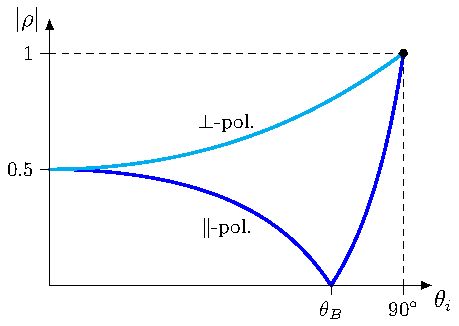
\includegraphics[width=0.5\linewidth]{img/1/Reflection-coef-function.pdf}
    \caption{Amplitude do coeficiente de reflexão em função do ângulo de incidência~\cite{silveirinha2023}}
    \label{fig:Reflection-coef-function}
\end{figure}

Retiramos as seguintes conclusões:
\begin{itemize}
    \item Para a incidência normal, as amplitudes de $\abs{\rho_{||}}$ e $\abs{\rho_{\perp}}$ são iguais.
    \item Com o aumento do ângulo de incidência, $\abs{\rho_{\perp}}$ aumenta monotonicamente, enquanto $\abs{\rho_{||}}$ diminui até ao \underline{ângulo de Brewster}, $\theta_B$.
    \item Para $\theta_i = \theta_B$, o coeficiente $\abs{\rho_{||}}$ é zero (assumindo ausência de perdas nos materiais).
    \item Para ângulos maiores que $\theta_B$, a magnitude de $\abs{\rho_{||}}$ volta a aumentar.
    \item Na incidência tangencial, onde $\theta_i \to 90^\circ$, ambos os coeficientes $\abs{\rho_{||}}$ e $\abs{\rho_{\perp}}$ tendem para um, o que indica uma reflexão total pela interface.
\end{itemize}

\begin{warning}
    É útil caracterizar $\rho_{||}$ e $\rho_{\perp}$ quando o meio 2 é um condutor elétrico perfeito. Como discutido \hyperref[warn:9]{anteriormente}, um condutor perfeito tem impedância $\eta_{PEC} = \eta_2 = 0$. Assim, para um condutor perfeito os dois coeficientes de reflexão são independentes do ângulo de incidência:
    \begin{equation}
        \rho_{\perp_{PEC}} = -1, \quad \rho_{\parallel_{PEC}} = +1.
    \end{equation}
\end{warning}

%//==============================--@--==============================//%
\renewcommand*{\thefootnote}{\fnsymbol{footnote}}
\subsubsection[Ângulo de Brewster]{Ângulo de Brewster\protect\footnotemark[2]}

Podemos obter uma expressão analítica para o ângulo de Brewster mantendo as suposições de meios sem perdas da secção anterior. Basta resolver a equação
\begin{equation}
    \rho_{\parallel} = \frac{\eta_1 \cos \theta_i - \eta_2 \cos \theta_t}{\eta_1 \cos \theta_i + \eta_2 \cos \theta_t} = 0
    \; \iff \;
    \eta_1 \cos \theta_i - \eta_2 \cos \theta_t = 0
    \; \implies \;
    \frac{1}{n_1} \cos \theta_i = \frac{1}{n_2} \cos \theta_t
\end{equation}
Através da 2\textordfeminine{} Lei de Snell, obtemos uma segunda equação que nos permitirá obter $\theta_i$ explicitamente:
\begin{equation}
    n_1 \sin \theta_i = n_2 \sin \theta_t
\end{equation}
Após uma simples manipulação algébrica pode ser visto que:
\begin{equation}
    \boxed{%
        \theta_B = \arctan\left( \frac{n_2}{n_1} \right)
    }
\end{equation}

\footnotetext[2]{%
    Uma relação geométrica curiosa é que, para $\theta_i = \theta_B$, os vetores $\mathbf{\hat{d}}^r$ e $\mathbf{\hat{u}}^i{\scriptstyle \parallel}$ são paralelos. Isto pode ser verificado observando que a condição de Brewster pode ser vista como $n_1 \sin \theta_B = n_2 \cos \theta_B$. Segundo a 2\textordfeminine{} Lei de Snell, $n_1 \sin \theta_B = n_2 \sin \theta_t$. Portanto, a condição de Brewster implica que $\cos \theta_B = \sin \theta_t$, o que só é possível se $\theta_B = 90^\circ - \theta_t$.
}
\renewcommand*{\thefootnote}{\fnsymbol{footnote}}

%//==============================--@--==============================//%
\clearpage
\begin{question}
    Considere uma onda eletromagnética plana circularmente polarizada para a direita, que se propaga no ar e incide numa camada dielétrica plana de grandes dimensões caracterizada por,
    $$
        \sigma = 0, \quad \mu_r = 1, \quad \epsilon_r = 5
    $$
    Suponha que o ângulo de incidência é de $45^\circ$ e que a densidade de potência da onda incidente junto à superfície de separação é de $10$ W/m$^2$.\\[3pt]
    a) Caracterize a onda refletida, quanto ao seu estado de polarização.\\[3pt]
    b) Determine a densidade de potência da onda refletida.

    \questionSep
    \textbf{Solução}: Vamos definir o ar como meio 1 e a camada dielétrica como meio 2. Assim,
    $$
        \text{meio 1:} \;
        \left\{
        \begin{aligned}
            \epsilon_1 &= \epsilon_0, \; \mu_1 = \mu_0 \\
            n_1 &= \sqrt{\mu_{r1} \epsilon_{r1}} = 1 \\
            \eta_1 &= \eta_0 \approx 377.0\; [\Omega]
        \end{aligned}\right.
        \qquad
        \text{meio 2:} \;
        \left\{
        \begin{aligned}
            \epsilon_2 &= 5\epsilon_0, \; \mu_2 = \mu_0 \\
            n_2 &= \sqrt{\mu_{r2} \epsilon_{r2}} = \sqrt{5} \\
            \eta_2 &= \eta_0/n_2 \approx 168.6\; [\Omega] 
        \end{aligned}\right.
    $$
    Uma vez que a onda incidente tem polarização circular para a direita, o rácio de polarização é
    $$
        p_{\text{inc}} = \frac{\underline{E}^{\text{inc}}_2}{\underline{E}^{\text{inc}}_1} = e^{-j\pi/2}
        \;\implies\;
        \underline{E}_2 = -j\underline{E}_1
    $$
    Podemos escrever a onda incidente como:
    $$
        \mathbf{\underline{E}}^{\text{inc}} = E_0 (\mathbf{\hat{u}}_{\perp} - j\mathbf{\hat{u}}_{\parallel})\, e^{-jk_0 \mathbf{\hat{d}}^i \cdot \mathbf{r}}
    $$
    Uma vez que $\mathbf{S}^{\text{inc}}_{\text{av}} = \norm{\mathbf{\underline{E}}^{\text{inc}}}^2/(2\eta_1)\, \mathbf{\hat{d}}^i$, podemos descobrir o valor de $E_0$ através da norma:
    $$
        \norm{\mathbf{S}^{\text{inc}}_{\text{av}}} = \frac{\norm{\mathbf{\underline{E}}^{\text{inc}}}^2}{2\eta_1}
        \;\iff\;
        2\eta_1\, \norm{\mathbf{S}^{\text{inc}}_{\text{av}}} = \norm{\mathbf{\underline{E}}^{\text{inc}}} = 2 E^2_0
        \;\implies\;
        E_0 = 61.4\; [\text{V/m}]
    $$
    Podemos finalmente escrever as equações dos campos refletido e transmitido:
    $$
        \begin{aligned}
            \mathbf{\underline{E}}^{\text{ref}} &= E_0 (\rho_{\perp} \mathbf{\hat{u}}_{\perp} - j\rho_{\parallel} \mathbf{\hat{u}}_{\parallel})\, e^{-jk_0 \mathbf{\hat{d}}^r \cdot \mathbf{r}} \\
            \mathbf{\underline{E}}^{\text{tx}} &= E_0 (\tau_{\perp} \mathbf{\hat{u}}_{\perp} - j\tau_{\parallel} \mathbf{\hat{u}}_{\parallel})\, e^{-j n_2 k_0 \mathbf{\hat{d}}^t \cdot \mathbf{r}}
        \end{aligned}
    $$
    Uma vez que $\theta_i = \pi/4$ e $\theta_t = \arcsin(n_1/n_2 \cdot \sin \theta_i)$, os coeficientes são dados por:
    $$
        \begin{aligned}
            \rho_{\perp} &= \frac{\eta_2 \cos \theta_i - \eta_1 \cos \theta_t}{\eta_2 \cos \theta_i + \eta_1 \cos \theta_t} = -\frac{1}{2} &\qquad \rho_{\parallel} &= \frac{\eta_1 \cos \theta_i - \eta_2 \cos \theta_t}{\eta_1 \cos \theta_i + \eta_2 \cos \theta_t} = \frac{1}{4} \\
            \tau_{\perp} &= 1 + \rho_{\perp} = \frac{1}{2} &\qquad \tau_{\parallel} &= \frac{\eta_2}{\eta_1} (1 + \rho_{\parallel}) = \frac{\sqrt{5}}{4}
        \end{aligned}
    $$
    Nestes moldes, podemos calcular a polarização das ondas refletida e transmitida:
    $$
        p_{\text{ref}} = \frac{\underline{E}^{\text{ref}}_2}{\underline{E}^{\text{ref}}_1} = \eqnmarkbox[violet]{pol-ref}{2 e^{j\pi/2}}, 
        \qquad
        p_{\text{tx}} = \frac{\underline{E}^{\text{tx}}_2}{\underline{E}^{\text{tx}}_1} = \eqnmarkbox[violet]{pol-tx}{0.89 e^{-j\pi/2}}
    $$
    \annotate[]{above, label below}{pol-ref}{pol. elíptica esq.}
    \annotate[]{above, label below}{pol-tx}{pol. elíptica dir.}

    \vspace{-1em}
    Segue o cálculo da densidade de potência de ambas:
    $$
        \norm{\mathbf{S}^{\text{ref}}_{\text{av}}} = \eqnmarkbox[violet]{Sav-ref}{\norm{\mathbf{S}^{\text{inc}}_{\text{av}}} \left(\frac{\abs{\rho_{\perp}}^2 + \abs{\rho_{\parallel}}^2}{2}\right)} = 1.56 \; \text{kW/m}^2,
        \qquad
        \norm{\mathbf{S}^{\text{tx}}_{\text{av}}} = \eqnmarkbox[violet]{Sav-tx}{\norm{\mathbf{S}^{\text{inc}}_{\text{av}}} \frac{\eta_1}{\eta_2}\left(\frac{\abs{\tau_{\perp}}^2 + \abs{\tau_{\parallel}}^2}{2}\right)} = 6.29 \; \text{kW/m}^2
    $$
    \annotatetwo{below, label above}{Sav-ref}{Sav-tx}{válido apenas quando a onda inc. tem pol. circular!}

    \footnotetext{\textbf{Nota}: \% potência refletida = $\norm{\mathbf{S}^{\text{ref}}_{\text{av}}} / \norm{\mathbf{S}^{\text{inc}}_{\text{av}}}$, mas \% potência transmitida = $(1-\norm{\mathbf{S}^{\text{ref}}_{\text{av}}} / \norm{\mathbf{S}^{\text{inc}}_{\text{av}}})$ e \textbf{não} $\norm{\mathbf{S}^{\text{tx}}_{\text{av}}} / \norm{\mathbf{S}^{\text{inc}}_{\text{av}}}$, atenção!}
\end{question}

%//==============================--@--==============================//%
\clearpage
\subsection{Reflexão Interna Total}

O ângulo incidente para o qual o ângulo de transmissão é igual a $90^\circ$ é denominado de ângulo critico e pode ser obtido através da \hyperref[subsubsec:lei-de-snell]{Lei de Snell}:
\begin{equation}
    \boxed{%
        \theta_c = \arcsin\left( \frac{n_2}{n_1} \right)
    }
\end{equation}
Quando o ângulo de incidência excede o ângulo crítico a onda sofre \textbf{reflexão interna total}, de modo que toda a energia incidente é totalmente refletida de volta para o meio de incidência.

Para $\theta_i > \theta_c$, os coeficientes de reflexão (para materiais sem perdas) têm exatamente amplitude unitária para ambas as polarizações:
\begin{equation}
\theta_i = \theta_r\qquad |\rho_{\parallel}| = |\rho_{\perp}| = 1, \quad \text{(reflexão interna total)}
\end{equation}
Este resultado pode ser depreendido para a polarização perpendicular. Admitindo $\cos\theta_t = -jC$ encontra-se que:
\begin{equation}
    \rho_{\perp} = \frac{\eta_2 \cos\theta_i + \eta_1 jC}{\eta_2 \cos\theta_i - \eta_1 jC}.
\end{equation}
Como o numerador e denominador da fração estão relacionados pela conjugação complexa, é imediato que $|\rho_{\perp}| = 1$.

Uma argumentação semelhante pode ser feita para $|\rho_{\parallel}|$.

\begin{question}
    Um tubarão nada debaixo de um barco circular de diâmetro $D$, conforme a figura apresentada. Determine o menor ângulo $2\theta_c$ dum cone imaginário dentro do qual o peixe pode nadar sem ser visto por um observador à superfície da água.
    \begin{figure}[H]
        \centering
        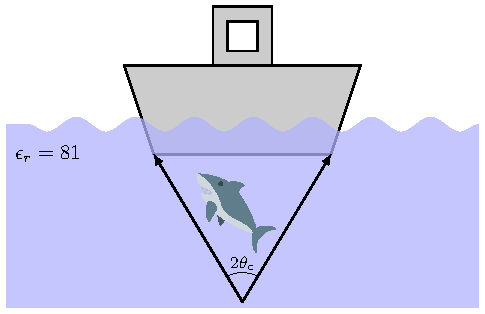
\includegraphics[width=.6\textwidth,keepaspectratio]{img/1/Shark.pdf}
    \end{figure}

    \vspace{-1em}
    \questionSep
    \textbf{Solução:} Para o peixe nadar dentro do cone sem ser visto, o ângulo dos feixes de luz que formam o cone têm de ser tais que ao incidirem entre a fronteira àgua/ar ocorre reflexão total, assim:
    $$
    \theta_\text{cone} \ge \theta_c, 
    \qquad
    \theta_c = \arcsin\left( \frac{n_\text{ar}}{n_\text{água}} \right) = 6.38^{\circ}\\
    $$
    Consequentemente,
    $$
        \boxed{\theta_\text{cone} = 6.38^{\circ}}
    $$
\end{question}


%//==============================--@--==============================//%